%%% LaTeX-Vorlage Version 1.8 %%%

% Grundlegende Dokumenteneigenschaften gemäß DHBW-Vorgaben
\documentclass[a4paper,fontsize=11pt,oneside,parskip=half,headings=normal,listof=nochaptergap]{scrreprt} 
% \usepackage{showframe} % nur für Kontrolle der Ränder 

%%% Präambel einbinden (mit Festlegungen gemäß DHBW-Vorgaben) %%%
%%% Präambel %%%
% hier sollten keine Änderungen erforderlich sein
%
\usepackage[utf8]{inputenc}   % Zeichencodierung UTF-8 für Eingabe-Dateien
\usepackage[T1]{fontenc}      % Darstellung von Umlauten im PDF

\usepackage{listings}         % für Einbindung von Code-Listings
\usepackage{xcolor}
\usepackage{booktabs}

\renewcommand\lstlistlistingname{Listingsverzeichnis}

\definecolor{codegreen}{rgb}{0,0.6,0}
\definecolor{codegray}{rgb}{0.5,0.5,0.5}
\definecolor{codepurple}{rgb}{0.58,0,0.82}
\definecolor{backcolour}{rgb}{0.95,0.95,0.92}

\lstdefinestyle{mystyle}{
  backgroundcolor=\color{backcolour},
  commentstyle=\color{codegreen},
  keywordstyle=\color{magenta},
  numberstyle=\tiny\color{codegray},
  stringstyle=\color{codepurple},
  basicstyle=\ttfamily\footnotesize,
  breakatwhitespace=false,
  breaklines=true,
  captionpos=b,
  keepspaces=true,
  numbers=left,
  numbersep=5pt,
  showspaces=false,
  showstringspaces=false,
  showtabs=false,
  tabsize=2,
  numberbychapter=false
}

\lstset{style=mystyle}

\lstset{literate=             % erlaubt Sonderzeichen in Code-Listings 
  {Ö}{{\"O}}1
{Ä}{{\"A}}1
{Ü}{{\"U}}1
{ß}{{\ss}}2
{ü}{{\"u}}1
{ä}{{\"a}}1
{ö}{{\"o}}1
{€}{{\euro}}1
}

\usepackage[
  inner=35mm,outer=15mm,top=25mm,
  bottom=20mm,foot=12mm,includefoot
]{geometry}                 % Einstellungen für Ränder
\usepackage{tabularx}
\usepackage[ngerman]{babel} % Spracheinstellungen Deutsch
\usepackage[babel,german=quotes]{csquotes} % deutsche Anf.zeichen
\usepackage{enumerate}      % anpassbare Nummerier./Aufz.
\usepackage{graphicx}       % Einbinden von Grafiken
\usepackage[onehalfspacing]{setspace} % anderthalbzeilig

\usepackage{blindtext}      % Textgenerierung für Testzwecke
\usepackage{color}          % Verwendung von Farbe 
\usepackage{pgfplots}      % für Diagramme
\pgfplotsset{compat=1.16}
\usepackage{tikz}
\usepackage{graphicx}
\usepackage{listings}
\usepackage{xcolor}
\definecolor{delim}{RGB}{20,105,176}
\definecolor{numb}{RGB}{106, 109, 32}
\definecolor{string}{rgb}{0.64,0.08,0.08}
\definecolor{backcolour}{rgb}{1,1,1}

\lstdefinelanguage{json}{
    basicstyle=\ttfamily\small\color{black},
    backgroundcolor=\color{backcolour},
    numbers=left,
    numberstyle=\small\color{gray},
    stepnumber=1,
    numbersep=8pt,
    showstringspaces=false,
    breaklines=true,
    frame=single,
    literate=
     *{0}{{{\color{numb}0}}}{1}
      {1}{{{\color{numb}1}}}{1}
      {2}{{{\color{numb}2}}}{1}
      {3}{{{\color{numb}3}}}{1}
      {4}{{{\color{numb}4}}}{1}
      {5}{{{\color{numb}5}}}{1}
      {6}{{{\color{numb}6}}}{1}
      {7}{{{\color{numb}7}}}{1}
      {8}{{{\color{numb}8}}}{1}
      {9}{{{\color{numb}9}}}{1}
      {\{}{{{\color{delim}{\{}}}}{1}
      {\}}{{{\color{delim}{\}}}}}{1}
      {[}{{{\color{delim}{[}}}}{1}
      {]}{{{\color{delim}{]}}}}{1}
      {,}{{{\color{delim}{,}}}}{1}
      {:}{{{\color{delim}{:}}}}{1},
    morestring=[b]",
    stringstyle=\color{red},   % Dies färbt alle Strings rot.
}
\usepackage[printonlyused]{acronym}        % für ein Abkürzungsverzeichnis

\usepackage[                % Biblatex
  backend=biber,
  bibstyle=_dhbw_authoryear,maxbibnames=99,
  citestyle=authoryear,
  uniquename=true, useprefix=true,
  bibencoding=utf8]{biblatex}
%kein Punkt am Ende bei \footcite
%http://www.golatex.de/footcite-ohne-punkt-am-schluss-t4865.html
\renewcommand{\bibfootnotewrapper}[1]{\bibsentence#1}


%Reihenfolge der Autorennamen
%   
% http://golatex.de/viewtopic,p,80448.html#80448
% Argumente: siehe http://texwelt.de/blog/modifizieren-eines-biblatex-stils/
\DeclareNameFormat{sortname}{% Bibliographie
  \ifnum\value{uniquename}=0 % Normalfall
  \ifuseprefix%
    {%
    \usebibmacro{name:family-given}
    {\namepartfamily}
    {\namepartgiveni}
    {\namepartprefix}
    {\namepartsuffixi}%
    }
    {%
    \usebibmacro{name:family-given}
    {\namepartfamily}
    {\namepartgiveni}
    {\namepartprefixi}
    {\namepartsuffixi}%
    }%
  \fi
  \ifnum\value{uniquename}=1% falls nicht eindeutig, abgek. Vorname 
    {%
    \usebibmacro{name:family-given}
    {\namepartfamily}
    {\namepartgiveni}
    {\namepartprefix}
    {\namepartsuffix}%
    }%
  \fi
  \ifnum\value{uniquename}=2% falls nicht eindeutig, ganzer Vorname 
    {%
    \usebibmacro{name:family-given}
    {\namepartfamily}
    {\namepartgiven}
    {\namepartprefix}
    {\namepartsuffix}%
    }%
  \fi
  \usebibmacro{name:andothers}}

\DeclareNameFormat{labelname}{% für Zitate
  \ifnum\value{uniquename}=0 % Normalfall
  \ifuseprefix%
    {%
    \usebibmacro{name:family-given}
    {\namepartfamily}
    {\empty}
    {\namepartprefix}
    {\namepartsuffixi}%
    }
    {%
    \usebibmacro{name:family-given}
    {\namepartfamily}
    {\empty}
    {\namepartprefixi}
    {\namepartsuffixi}%
    }%
  \fi
  \ifnum\value{uniquename}=1% falls nicht eindeutig, abgek. Vorname 
    {%
    \usebibmacro{name:family-given}
    {\namepartfamily}
    {\namepartgiveni}
    {\namepartprefix}
    {\namepartsuffix}%
    }%
  \fi
  \ifnum\value{uniquename}=2% falls nicht eindeutig, ganzer Vorname 
    {%
    \usebibmacro{name:family-given}
    {\namepartfamily}
    {\namepartgiven}
    {\namepartprefix}
    {\namepartsuffix}%
    }%
  \fi
  \usebibmacro{name:andothers}}


\DeclareFieldFormat{extrayear}{% = the 'a' in 'Jones 1995a'
  \iffieldnums{labelyear}
  {\mknumalph{#1}}
  {\mknumalph{#1}}}

\renewcommand*{\multinamedelim}{\addslash}
\renewcommand*{\finalnamedelim}{\addslash}
\renewcommand*{\multilistdelim}{\addslash}
\renewcommand*{\finallistdelim}{\addslash}

\renewcommand{\nameyeardelim}{~}

% Literaturverzeichnis: Doppelpunkt zwischen Name (Jahr): Rest 
% http://de.comp.text.tex.narkive.com/Tn1HUIXB/biblatex-authoryear-und-doppelpunkt
\renewcommand{\labelnamepunct}{\addcolon\addspace}

% damit die Darstellung für Vollzitate von Primärquellen in 
% Fußnoten später auf "nicht fett" geändert werden kann 
% (nur für Zitate von Sekundärliteratur relevant)
\newcommand{\textfett}[1]{\textbf{#1}}

% für Zitate von Sekundärliteratur:
\newcommand{\footcitePrimaerSekundaer}[4]{%
  \renewcommand{\textfett}[1]{##1}%
  \footnote{\fullcite[#2]{#1}, zitiert nach \cite[#4]{#3}}%  
  \renewcommand{\textfett}[1]{\textbf{##1}}%
}

% Im Literaturverzeichnis: Autor (Jahr) fett
\renewbibmacro*{author}{%
  \ifboolexpr{%
    test \ifuseauthor%
    and
    not test {\ifnameundef{author}}
  }
  {\usebibmacro{bbx:dashcheck}
    {\bibnamedash}
    {\usebibmacro{bbx:savehash}%
      \textfett{\printnames{author}}%
      \iffieldundef{authortype}
      {\setunit{\addspace}}
      {\setunit{\addcomma\space}}}%
    \iffieldundef{authortype}
    {}
    {\usebibmacro{authorstrg}%
      \setunit{\addspace}}}%
  {\global\undef\bbx@lasthash
    \usebibmacro{labeltitle}%
    \setunit*{\addspace}}%
  \textfett{\usebibmacro{date+extrayear}}}

% Sonderfall: Quelle ohne Autor, aber mit Herausgeber
% Name des Herausgebers wird fett gedruckt
\renewbibmacro*{bbx:editor}[1]{%
  \ifboolexpr{%
    test \ifuseeditor%
    and
    not test {\ifnameundef{editor}}
  }
  {\usebibmacro{bbx:dashcheck}
    {\bibnamedash}
    {\textfett{\printnames{editor}}%
      \setunit{\addcomma\space}%
      \usebibmacro{bbx:savehash}}%
    \usebibmacro{#1}%
    \clearname{editor}%
    \setunit{\addspace}}%
  {\global\undef\bbx@lasthash
    \usebibmacro{labeltitle}%
    \setunit*{\addspace}}%
  \textfett{\usebibmacro{date+extrayear}}}

% Anpassungen für deutsche Sprache
\DefineBibliographyStrings{ngerman}{%
  nodate = {{o.J.}},
  urlseen = {{Abruf:}},
  ibidem = {{ebenda}}
}

% keine Anführungszeichen beim Titel im Literaturverzeichnis
\DeclareFieldFormat[article,book,inbook,inproceedings,manual,misc,phdthesis,thesis,online,report]{title}{#1\isdot}

\newcommand{\literaturverzeichnis}{%
  % nur Literaturverzeichnis
  % (als eigenes Kapitel)
  \phantomsection
  \addcontentsline{toc}{chapter}{Literaturverzeichnis}
  \spezialkopfzeile{Literaturverzeichnis}
  \defbibheading{lit}{\chapter*{Literaturverzeichnis}}
  \label{chapter:quellen}
  \printbibliography[heading=lit,notkeyword=ausblenden]
} % mit DHBW-spezifischen Einstellungen

\usepackage[hidelinks]{hyperref}       % URL-Formatierung, klickbare Verweise

\usepackage{tocloft}        % für Verzeichnis der Anhänge


\newcounter{anhcnt}
\setcounter{anhcnt}{0}
\newlistof{anhang}{app}{}

\newcommand{\anhang}[1]{%
  \refstepcounter{anhcnt}
  \setcounter{anhteilcnt}{0}
  \section*{Anhang \theanhcnt: #1}
  \addcontentsline{app}{section}{\protect\numberline{Anhang \theanhcnt}#1}\par
}

\newcounter{anhteilcnt}
\setcounter{anhteilcnt}{0}

\newcommand{\anhangteil}[1]{%
  \refstepcounter{anhteilcnt}
  \subsection*{Anhang~\arabic{anhcnt}/\arabic{anhteilcnt}: #1}
  \addcontentsline{app}{subsection}{\protect\numberline{Anhang \theanhcnt/\arabic{anhteilcnt}}#1}\par
}

\renewcommand{\theanhteilcnt}{Anhang \theanhcnt/\arabic{anhteilcnt}}

% vgl. S. 4 Paket-Beschreibung tocloft 	
% Einrückungen für Anhangverzeichnis
\makeatletter
\newcommand{\abstaendeanhangverzeichnis}{
  \renewcommand*{\l@section}{\@dottedtocline{1}{0em}{5.5em}}
  \renewcommand*{\l@subsection}{\@dottedtocline{2}{2.3em}{6.5em}}
}
\makeatother

% Abbildungs- und Tabellenverzeichnis
% Bezeichnungen
\renewcaptionname{ngerman}{\figurename}{Abb.}
\renewcaptionname{ngerman}{\tablename}{Tab.}
% Einrückungen
\makeatletter
\renewcommand*{\l@figure}{\@dottedtocline{1}{0em}{2.3em}}
\renewcommand*{\l@table}{\@dottedtocline{1}{0em}{2.3em}}
\makeatother


\usepackage{chngcntr}                % fortlaufende Zähler für Fußnoten, Abbildungen und Tabellen
\counterwithout{figure}{chapter}
\counterwithout{table}{chapter}
\counterwithout{footnote}{chapter}

\usepackage[automark]{scrlayer-scrpage}
%% Definitionen für Kopf- und Fußzeile auf normalen Seiten
\defpagestyle{kopfzeile}
{% Kopfdefinition
  (\textwidth,0pt)    % Länge der oberen Linie,Dicke der oberen Linie       
  {} % Definition für linke Seiten im doppelseitigen Layout
    {} % Definition für rechte Seiten im doppelseitigen Layout      
    {  % Definition für Seiten im einseitigen Layout
      \makebox[0pt][l]{\rightmark}% 
      \makebox[\linewidth]{}% 
    }
  (\textwidth, 0.4pt) % Untere Linienlänge, Untere Liniendicke
}
{% Fußdefinition
  (\textwidth,0pt)    % Obere Linienlänge, Obere Liniendicke
  {} % Definition für linke Seiten im doppelseitigen Layout
    {} % Definition für rechte Seiten im doppelseitigen Layout
    {  % Definition für Seiten im einseitigen Layout
      \makebox[\linewidth]{}%
      \makebox[0pt][r]{\pagemark}%
    }
  (\textwidth, 0pt)   % Länge der unteren Linie,Dicke der unteren Linie
}

%% Definitionen für Kopf- und Fußzeile auf ersten Seiten eines Kapitels
\defpagestyle{kapitelkopfzeile}
{% Kopfdefinition
  (\textwidth,0pt)    % Länge der oberen Linie,Dicke der oberen Linie       
  {} % Definition für linke Seiten im doppelseitigen Layout
    {} % Definition für rechte Seiten im doppelseitigen Layout      
    {}  % Definition für Seiten im einseitigen Layout
  (\textwidth, 0pt) % Untere Linienlänge, Untere Liniendicke
}
{% Fußdefinition
  (\textwidth,0pt)    % Obere Linienlänge, Obere Liniendicke
  {} % Definition für linke Seiten im doppelseitigen Layout
    {} % Definition für rechte Seiten im doppelseitigen Layout
    {  % Definition für Seiten im einseitigen Layout
      \makebox[\linewidth]{}%
      \makebox[0pt][r]{\pagemark}%
    }
  (\textwidth, 0pt)   % Länge der unteren Linie,Dicke der unteren Linie
}

%% Definitionen für Kopf- und Fußzeile im Anhang und bei Quellenverzeichnisse
\newcommand{\spezialkopfzeileBezeichnung}{}
\defpagestyle{spezialkopfzeile}
{% Kopfdefinition
  (\textwidth,0pt)    % Länge der oberen Linie,Dicke der oberen Linie       
  {} % Definition für linke Seiten im doppelseitigen Layout
    {} % Definition für rechte Seiten im doppelseitigen Layout      
    {  % Definition für Seiten im einseitigen Layout
      \makebox[0pt][l]{\spezialkopfzeileBezeichnung}% 
      \makebox[\linewidth]{}% 
    }
  (\textwidth, 0.4pt) % Untere Linienlänge, Untere Liniendicke
}
{% Fußdefinition
  (\textwidth,0pt)    % Obere Linienlänge, Obere Liniendicke
  {} % Definition für linke Seiten im doppelseitigen Layout
    {} % Definition für rechte Seiten im doppelseitigen Layout
    {  % Definition für Seiten im einseitigen Layout
      \makebox[\linewidth]{}%
      \makebox[0pt][r]{\pagemark}%
    }
  (\textwidth, 0pt)   % Länge der unteren Linie,Dicke der unteren Linie
}

\newcommand\spezialkopfzeile[1]{%
  \renewcommand\spezialkopfzeileBezeichnung{#1}
  \pagestyle{spezialkopfzeile}
}

% Standard-Pagestyle auswählen
\pagestyle{kopfzeile}

% keine Kopfzeile anzeigen auf Seiten, auf denen ein 
% Kapitel beginnt oder das Inhalts-/Abbildungs-/Tabellenverzeichnis steht 
\renewcommand{\chapterpagestyle}{kapitelkopfzeile}
\tocloftpagestyle{kapitelkopfzeile}

		 % für schöne Kopfzeilen 

\usepackage{textcomp}            % erlaubt EUR-Zeichen in Eingabedatei
\usepackage{eurosym}             % offizielles EUR-Symbol in Ausgabe
\renewcommand{\texteuro}{\euro}  % ACHTUNG: nach hyperref aufrufen!

\usepackage{scrhack}             % stellt Kompatibilität zw. KOMA-Script
% (scrreprt) und anderen Paketen her

% Anpassung der Abstände bei Kapitelüberschriften
% (betrifft auch Inhalts-, Abbildungs- und Tabellenverzeichnis)
\renewcommand*\chapterheadstartvskip{\vspace*{-\topskip}}
\newcommand{\myBeforeTitleSkip}{1mm}
\newcommand{\myAfterTitleSkip}{10mm}
\setlength\cftbeforetoctitleskip{\myBeforeTitleSkip}
\setlength\cftbeforeloftitleskip{\myBeforeTitleSkip}
\setlength\cftbeforelottitleskip{\myBeforeTitleSkip}

\setlength\cftaftertoctitleskip{\myAfterTitleSkip}
\setlength\cftafterloftitleskip{\myAfterTitleSkip}
\setlength\cftafterlottitleskip{\myAfterTitleSkip}
%%% Ende der Präambel %%%


%%% Name der eigenen Literatur-Datenbank (ggf. anpassen) %%%
\bibliography{includes/literatur.bib}

\begin{document}
%%% Deckblatt einbinden %%% 
% Anpassungen nötig (Name, Titel etc.)
% HIER EDITIEREN: 
% Typ der Arbeit (für Deckblatt und Metadaten)
% - bitte Zutreffendes auswählen
%\newcommand{\typMeinerArbeit}{1. Projektarbeit}
%\newcommand{\typMeinerArbeit}{2. Projektarbeit}
%\newcommand{\typMeinerArbeit}{Seminararbeit}
\newcommand{\typMeinerArbeit}{Bachelorarbeit}

% Thema der Arbeit (für ehrenwörtliche Erklärung, ohne Umbrüche)
% HIER EDITIEREN: 
\newcommand{\themaMeinerArbeit}{Document Understanding Transformers in der Dokumentenverarbeitung}

% Vorname, Name der Autorin/des Autors (für Titelseite und Metadaten)
% HIER EDITIEREN:
\newcommand{\meinName}{Marc Novak}

\thispagestyle{empty}

\begin{spacing}{1}
  \begin{center}
    ~\vspace{0mm}

    % HIER EDITIEREN: Titel der Arbeit
    {\sffamily
      \LARGE
      % \Large  % bei sehr langen Titeln ggf. etwas kleinere Schriftart wählen
      \textbf{Document Understanding Transformers in der Dokumentenverarbeitung}

      \bigskip
      \textbf{}
    }


    \vspace{15mm}

    % Typ wird automatisch eingefügt (oben festlegen)
    {\Large \typMeinerArbeit}

    \vspace{1cm}

    % HIER ggf. EDITIEREN
    vorgelegt am \today

    \vspace{15mm}

    Fakultät Wirtschaft
    \medskip

    Studiengang Wirtschaftsinformatik
    \medskip

    % HIER EDITIEREN: Kurs eintragen
    Kurs WI2021G

    \vspace{10mm}

    von

    \vspace{10mm}

    % Vorname und Name wird automatisch eingefügt (oben festlegen) 
    {\large\textsc{\meinName}}

    \vspace{10mm}
  \end{center}

  \vfill

  % HIER EDITIEREN: Name des Unternehmens, Name der Betreuerin/des Betreuers
  \begin{tabular}{ll}
    Betreuer in der Ausbildungsstätte:        & DHBW Stuttgart:                                                    \\
    \hspace{0.4\linewidth}                    &                                                                    \\
    ELO Digital Office GmbH & $\langle$ Titel, Vorname und Nachname $\rangle$                    \\
    Dr. Konstantin Hauch
                                              & $\langle$ der/des wissenschaftlichen Betreuerin/Prüferin $\rangle$ \\
    Teamleiter Team KI                                                     \\
    \\
    Unterschrift der Betreuerin/des Betreuers                                                                      \\
  \end{tabular}


  \vspace{1cm}
  %(etwas Platz für die Unterschrift der Betreuerin/des Betreuers aus der Ausbildungsstätte)
\end{spacing}

% falls ein Vertraulichkeitsvermerk erforderlich ist,
% die Kommentarzeichen in den nachfolgenden Zeilen entfernen:

%\begin{center}
%\small
%\textbf{Vertraulichkeitsvermerk}:
%Der Inhalt dieser Arbeit darf weder als Ganzes noch in Auszügen \\
%Personen außerhalb des Prüfungs- und Evaluationsverfahrens zugänglich gemacht werden, sofern keine anders lautende Genehmigung des Dualen Partners vorliegt. 
%\end{center}

% Meta-Daten für PDF-Datei basierend auf obigen Angaben
\hypersetup{pdftitle={\themaMeinerArbeit}}
\hypersetup{pdfauthor={\meinName}}
\hypersetup{pdfsubject={\typMeinerArbeit\ DHBW Stuttgart \the\year}}


%%% Umstellung der Seiten-Nummerierung auf i, ii, iii ... %%%
\pagenumbering{Roman}
\cleardoublepage

%%% Inhalts-, Abbildungs-, Tabellenverzeichnisse %%%
% sollen einzeilig gesetzt werden, um Platz zu sparen 
\begin{spacing}{1}
  \tableofcontents
  \clearpage
  \chapter*{Abkürzungsverzeichnis}
\addcontentsline{toc}{chapter}{Abkürzungsverzeichnis}

\begin{acronym}[DHBW]
  % Argument definiert die Breite der ersten Spalte anhand des längsten vorkommenden Eintrags
  \acro{CRM}{Customer Relationship Management}
  \acro{DHBW}{Duale Hochschule Baden-Württemberg}
  \acro{IEEE}{Institute of Electrical and Electronics Engineers}
  \acro{ITIL}{IT Infrastructure Library}
  \acro{RoI}{Return-On-Invest}
  \acro{UCS}{Universal Character Set}
  \acro{UTF-8}{8-Bit UCS Transformation Format}
\end{acronym}

\vspace{2em}


  \clearpage
  \thispagestyle{kapitelkopfzeile}
  \listoffigures
  \phantomsection
  \addcontentsline{toc}{chapter}{Abbildungsverzeichnis} % Abb.verz. ins Inh.verz. aufnehmen

  \clearpage
  \listoftables
  \phantomsection
  \addcontentsline{toc}{chapter}{Tabellenverzeichnis}   % Tab.verz. ins Inh.verz. aufnehmen
  \clearpage
  \lstlistoflistings
  \addcontentsline{toc}{chapter}{Listingsverzeichnis}   % Lst.verz. ins Inh.verz. aufnehmen
\end{spacing}

%%% Umstellung der Seiten-Nummerierung auf 1, 2, 3 ... %%%
\cleardoublepage
\pagenumbering{arabic}

%%% Ihr eigentlicher Inhalt %%%
% Empfehlung: strukturieren Sie Ihren Text in einzelnen Dateien 
% und binden Sie diese hier mit \input{includes/dateiname.tex} ein
\chapter{Einleitung}

In den vergrangenen Jahren hat \ac{KI} in Unternehmen zunehmend an Bedeutung gewonnen. Seit 2019 verzeichnet der KI-Software Markt einen hohes Wachstum. Es wird davon ausgegangen, dass dieses Wachstum bis 2025 mit über 26 \% pro Jahr anhalten wird. \footcites[Vgl.][]{howarth_57_2024} Die Anwendungsbereiche von KI-Systemen sind vielfältig und reichen von der Automatisierung von Prozessen, über die Analyse von großen Datenmengen bis hin zur Vorhersage von zukünftigen Ereignissen.

Einer der beliebtesten Anwendungsbereiche von KI-Systemen ist die Dokumentenverarbeitung. Eine Befragung von 1420 IT-Fachkräften ergab, dass 28 \% der zugehörigen Unternehmen KI-Systeme zur Dokumentenverarbeitung einsetzen (s. Abb. \ref{fig:ai_tech_distribution}). \footcites[Vgl.][]{rackspace_most_2023} Die Dokumentenverarbeitung umfasst die Extraktion von Informationen, die Klassifizierung und die automatisierte Verarbeitung von Dokumenten.\footcites[Vgl.][S.1]{esposito_intelligent_2005} Die Verarbeitung von Dokumenten ist in vielen Unternehmen ein zeitaufwändiger Prozess, der durch den Einsatz von KI-Systemen automatisiert und beschleunigt werden kann.\footcites[Vgl.][S.11]{dutt_now_2024}

\pgfplotsset{compat=1.17} % Use the version of pgfplots you have installed

\begin{figure}[htb]
    \centering
\begin{tikzpicture}
    \begin{axis}[
        xbar, % Horizontal bars
        xmin=0, xmax=60, % Set the minimum and maximum x-coordinates
        width=11cm, height=9cm, % Width and height of the plot
        enlarge y limits=0.1, % Add some space between bars
        xlabel={Share of respondents in \%}, % Label for the x-axis
        symbolic y coords={
            Speech recognition,
            Image recognition,
            Facial recognition,
            Sales and marketing analytics,
            Document processing,
            Intelligent search,
            Recommender systems,
            Natural language processing,
            Predictive maintenance,
            Customer engagement,
            Computer vision
        },
        ytick=data, % Use the data for y-ticks
        nodes near coords,
        nodes near coords align={anchor=west}, % Add the percentage labels near the bars% Align the labels horizontally
        point meta=explicit symbolic % The meta data is explicitly given as symbolic text
    ]
    \addplot [draw=blue,fill=blue!30 ] coordinates {
        (51,Computer vision)[51\%]
        (47,Customer engagement)[47\%]
        (43,Predictive maintenance)[43\%]
        (38,Natural language processing)[38\%]
        (34,Recommender systems)[34\%]
        (31,Intelligent search)[31\%]
        (28,Document processing)[28\%]
        (26,Sales and marketing analytics)[26\%]
        (23,Facial recognition)[23\%]
        (18,Image recognition)[18\%]
        (13,Speech recognition)[13\%]};
    \end{axis}
\end{tikzpicture}
\caption[Gängigste Verwendungszwecke von KI in Unternehmen]{Gängigsten Verwendungszwecke von KI in Unternehmen\footnotemark} % Caption for the figure
    \label{fig:ai_tech_distribution} % Label for referencing the figure
\end{figure}
\footnotetext{Entnommen aus: \cite{rackspace_most_2023}}

Die Verarbeitung von gescannten Dokumenten, insbesondere von Rechnungen ist ein integraler Bestandteil der Dokumentenverarbeitung. Der Einsatz von \ac{OCR} ermöglicht die Digitalisierung und elektronische Weiterverarbeitung dieser Dokumente. Jeoch ist die Zuordnung der erkannten Zeichenketten zu interpretierbaren Metadaten oft von manueller Nachbearbeitung oder von regulären Ausdrücken abhängig. Eine weitere Hürde, welche sich bei der Extraktion von Informationen aus Rechnungen zeigt, sind die sehr heterogenen Vorlagen und Layouts, welche in der Verarbeitung zu Ungenauigkeiten führen kann. Die OCR kann hier nicht mehr sicher die erkannten Werte den entsprechenden Labeln zuordnen.\footcites[Vgl.][S.1]{rahal_information_2018} Die DMS-Software \ac{ELO} von ELO verarbeitet Rechnungen zurzeit mittels OCR. Die Anwendung von Transformer-Modellen, im Bereich des \ac{VDU} ermöglicht eine direkte kontextbasierte Weiterverarbeitung der Rechnungen.\footcites[Vgl.][S.1]{kim_ocr-free_2021}

Diese Arbeit untersucht neue Transformer-Modelle im Bereich des VDU. Es wird analysiert, wie diese Modelle, die ihren Ursprng in der natürlichen Sprachverarbeitung haben, auf die Interpretation visueller (layoutbasierter) und textueller Elemente in Dokumenten angewandt werden können. Weiterhin wird ein OCR-freier \ac{Donut} untersucht, um die Limitierungen von OCR bezüglich Laufzeit und Fehleranfälligkeit zu überwinden.\footcites[Vgl.][S.1]{kim_ocr-free_2021} Diese Arbeit umfasst die Bereitstellung einer Pipeline, welche vom Modelltraining des Donuts bis zur Endanwendung im Unternehmen ELO Digital Office GmbH reicht. 
Das Ziel dieser Arbeit ist es, die Anwendbarkeit von Transformer-Modellen im Bereich des \ac{VDU} zu untersuchen und die Leistungsfähigkeit der Pipeline zu evaluieren um folgende Forschungsfrage zu beantworten:
\begin{center}
    \emph{Kann die Anwendung von Document Understanding Transformer Modellen die Effizienz und Genauigkeit der Rechnungsverarbeitung im Vergleich zu bestehenden OCR-basierten Modellen steigern?}
\end{center} 
Um diese Frage zu beantworten wird anhand eines Benchmarks (detaillierte Beschreibung des Aufbaus folgt in Kapitel 3) die Leistungsfähigkeit der Donut-basierten Pipeline mittels diverser Metriken bemessen und zur Leistungsfähigkeit von OCR-basierten Modellen verglichen. Daher ist die Arbeit folgedermaßen strukturiert: \\Zunächst werden in Kapitel 2 die Grundlagen der Dokumentenverarbeitung und der Transformer-Modelle erläutert. In Kapitel 3 werden die zu untersuchenden Modelle ausgewählt. Des weiteren werden der experimentelle Ansatz und der Aufbau der Testumgebung und Datensätze beschrieben. In Kapitel 4 wird die Entwicklung der Pipeline und die Implementierung des Donut dargestellt. Kapitel 5 präsentiert die Ergebnisse des Experiments. Kapitel 6 diskutiert die Ergebnisse und zieht Schlussfolgerungen. Eine Zusammenfassung und ein Ausblick auf zukünftige Arbeiten schließen die Arbeit in Kapitel 7 ab. Mit dieser Strukturierung als Ausgangspunkt, folgt nun die detaillierte Betrachtung der Grundlagen der Dokumentenverarbeitung und der Transformer-Modelle in Kapitel 2.

\chapter{Theoretischer Hintergrund}
Im folgenden Kapitel werden die theoretischen Grundlagen für diese Arbeit erläutert, um ein Verständnis für die verwendeten Begriffe und Technologien zu schaffen. Zunächst wird ein kurzer Überblick über die \ac{OCR} gegeben. Anschließend werden die Grundlagen der Transformer-Modelle erläutert. Des Weiteren werden die Details des \ac{Donut} genauer betrachtet, um ein Verständnis für die Funktionsweise des Modells im Vergleich zu herkömmlichen Methoden zu schaffen.

\section{Grundlagen der OCR}
Dieser Abschnitt betrachtet die grundlegende Funktionsweise und die Anwendungsbereiche von OCR-Systemen, da auch heute noch die meisten Modelle der Dokumentenverarbeitung auf eine OCR für den textuellen Input angewiesen sind (siehe dazu bspw. LayoutLM3\footcites[Vgl. dazu ausführlich][]{huang_layoutlmv3_2022}, ERNIE\footcites[Vgl. dazu ausführlich][]{peng_ernie-layout_2022}, FastStrucText\footcites[Vgl. dazu ausführlich][]{zhai_fast-structext_2023} etc.). Der Abschnitt bietet einen grundlegenden Überblick über das Thema. Auf ein tieferes Verständnis und eine detaillierte Betrachtung der Funktionsweise von OCR-Systemen wird in dieser Arbeit nicht eingegangen, da der Fokus auf der Anwendung von Transformer-Modellen im Bereich der Dokumentenverarbeitung liegt. Dennoch darf die Relevanz von OCR-Systemen nicht unterschätzt werden, da sie in vielen \ac{SOTA}-Modellen immer noch als Basis für die Textextraktion dienen. 

Häufig liegen Informationen in handschriftlicher oder gedruckter Form vor. Diese Informationen können durch Scans als Bilder in Computern gespeichert werden, jedoch ist die weiterverarbeitung der Informationen schwierig. Das System kann nicht ohne weiteres auf den Text in den erfassten Bildern zugreifen, bzw. diesen Lesen. Das Ziel von OCR ist es, Text aus Bildern zu extrahieren. OCR-Systeme sind in der Lage, Text aus gescannten Dokumenten, Fotos oder anderen Bildern zu extrahieren und in maschinenlesbaren Text umzuwandeln. In einem solchen Format können die Informationen weiterverarbeitet und analysiert werden. Somit ermöglicht es OCR einer Maschine, Texte automatisch zu erkennen.\footcites[Vgl.][S.244]{hamad_detailed_2016}

Für eine hohe Qualität und Genauigkeit der Zeichenerkennung erwarten OCR-Systeme eine hohe Qualität der Eingabebilder. Die Qualität der Eingabebilder ist ein entscheidender Punkt für die Genauigkeit der Zeichenerkennung. Einige Faktoren stellen Herausforderungen für die OCR dar, darunter die Szenenkomplexität, ungleiche Beleuchtungsbedingungen, Verzerrungen, Unschärfe und Abbau, Aspektverhältnisse, die Kippung, die Schriftart und mehrsprachige Umgebungen.\footcites[Vgl.][S.245]{hamad_detailed_2016} Die Herausforderungen erfordern fortgeschrittene Algorithmen und Techniken, einschließlich maschinellem Lernen und künstlicher Intelligenz, um die Erkennungsrate zu verbessern. Diese Herausforderungen versucht das Donut-Modell zu überwinden, indem es auf Transformer-Modellen basiert und somit die Limitierungen von OCR-Systemen umgeht.\footcites[Vgl.][S.1]{kim_ocr-free_2021} Um die Ergebnisse von OCR-Systemen zu verbessern werden in der Literatur verschiedene Ansätze vorgeschlagen. Nguyen et. al. schlagen die Verwendung von BERT vor. Als kontextbasiertes Sprachmodell kann BERT die Genauigkeit der OCR-Systeme verbessern, indem es die Kontextinformationen der Wörter berücksichtigt. Die Autoren zeigen, dass BERT die Genauigkeit der OCR-Systeme durch Fehlererkennung und Korrektur verbessern kann.\footcites[Vgl.][S.335 f.]{nguyen_neural_2020} BERT und seine Derivate werden noch heute in vielen \ac{SOTA}-Modellen für die Textextraktion verwendet.\footcites[Vgl. dazu ausführlich][S.4084 ff.]{huang_layoutlmv3_2022} \footcites[Vgl. dazu ausführlich][S.2 ff.]{garncarek_lambert_2020}

Die Funktionsweise von OCR-Systemen kann in sechs Phasen unterteilt werden. Diese Phasen umfassen die Vorverarbeitung, die Segmentierung, die Normalisierung, die Merkmalsextraktion, die Klassifikation und die Postverarbeitung. Das Ziel der Vorverarbeitung ist es, das Eingabebild zu verbessern und zu bereinigen. Die Segmentierung ist der Prozess, bei dem das Bild in einzelne Zeichen oder Wörter aufgeteilt und vom Hintergrund des Bildes getrennt wird. Sie stellt die kritische und maßgebliche Komponente eines OCR-Systems dar. Die Normalisierung ist der Prozess, bei dem die Segmentierungsergebnisse in eine standardisierte Form gebracht werden. In der Merkmalsextraktionsphase extrahiert das System relevante Merkmale von Objekten oder Alphabeten und wandelt diese zu Merkmalsvektoren um. In der Klassifikationsphase werden die Eingaben unterschiedlichen Klassen zugeordnet.\footcites[Vgl.][S.244]{hamad_detailed_2016} Beispielsweise wird in der Klassifikationsphase die Rechnungsnummer einer Klasse \emph{Invoice-Nr.} zugeordnet und das Datum der Klasse \emph{Date}. Es gibt diverse Werkzeuge, um die Klassifikation durchzuführen. Laut Dongre u.a. ist das \emph{Character Classification Problem} verwandt mit der heuristischen Logik, da Menschen Zeichen und Dokumente durch Erfahrung und Lernen erkennen können. Da Neuronale Netze ebenfalls von heuristischer Natur sind, sollten sie sich besonders gut für solche Probleme eignen. \footcites[Vgl.][S.11]{dongre_review_2010} Hier bleibt jedoch unbeachtet, dass die Eignung auch von der Qualität des Netzes selbst abhängt, welche wiederrum von der Qualität der Trainingsdaten abhängig ist.\footcites[Vgl.][S.851]{kavzoglu_increasing_2009} Daher eignet sich das Neuronale Netz als Klassifikator nur dann besonders gut, wenn die Trainingsdaten von hoher Qualität sind und das Netz in der Klassifikation eine hohe Genauigkeit aufweist. In der Postverarbeitung werden abschließend die Klassifikationsergebnisse weiterverarbeitet und korrigiert, um die Genauigkeit des erkannten Textes zu erhöhen.\footcites[Vgl.][S.246 f.]{hamad_detailed_2016} Hier wird das zuvor genannte BERT-Modell eingesetzt, um die Genauigkeit der OCR-Systeme zu verbessern.\footcites[Vgl.][S.335 f.]{nguyen_neural_2020}

Die Anwendungsbereiche der OCR sind vielfältig. Sie reichen von der Digitalisierung von Dokumenten in der Rechtsbranche über die Verarbeitung von Checks in Banken bis ins Gesundheitswesen. Der für diese Arbeit relevante Verwendungszweck ist die Verarbeitung von Rechnungen. OCR-Systeme werden in vielen Organisationen eingesetzt, um Rechnungen zu digitalisieren und diese so zu überwachen.\footcites[Vgl.][S.247 f.]{hamad_detailed_2016}

\section{Transformer-Modelle}
Im Folgenden soll ein Verständnis für die Transformer-Modelle geschaffen werden, welche wiederrum die Grundlage für Donut bilden. Dabei werden zunächst die Herkunft und Relevanz der Transformer-Modelle (folgend auch Transformer genannt) erläutert. Anschließend wird die Funktionsweise der Modelle genauer betrachtet. Dabei werden Schlüsselkonzepte wie die Aufmerksamkeit und das Positional Encoding, sowie die Architektur der Modelle erläutert. Seit der Einführung der Transformer in 2017 durch Vaswani et al. \footcites{vaswani_attention_2017} sind diese zum de facto Standard für eine Reihe verschiedener \ac{NLP} Aufgaben geworden. \ac{NLP} ist ein Teilbereich der Informatik, welcher es ermöglchen soll Computer Sprache auf eine \emph{natürliche} Art und Weise zu verstehen, so wie Menschen. Typischerweise refferenziert dies Aufgaben wie das Verstehen von Gefühlen in Texten, die Spracherkennung und das generieren von Antworten auf Fragen. \footcites[Vgl.][S.1]{beysolow_ii_applied_2018} Mittlerweile werden Transformer in den bekanntesten und meist genutzen Modellen der Welt verwendet, darunter BERT und GPT. \footcites[Vgl.][S. 1]{tunstall_natural_2022} Die beachtliche Leistungsfähigkeit der Transformer zeigt sich in den Benutzerzahlen von ChatGPT (ein ChatBot von OpenAI welcher auf den Transformer-Modellen basiert). Innerhalb von fünf Tage nach der Veröffentlichung des Modells hatte ChatGPT bereits eine Millionen Nutzer. Im Vergleich dazu brauchte Instagram zwei und halb Monate, um die gleiche Anzahl an Nutzern zu erreichen. \footcites[Vgl.][]{buchholz_infographic_2023} Den Status quo, vor der Entwicklung der Transformer, bildeten die \ac{RNN} und \ac{LSTM} Modelle. Transformer erzielen sowohl in der Leistungsfähigkeit als auch in den Trainingskosten bessere Ergebnisse als seine Vorgänger. \footcites[Vgl.][S. 1]{tunstall_natural_2022}

\subsection{Konzepte und Terminologie der Transformer-Modelle}
%TODO: Complete Chapter: Self-Attention, Multi-Head Attention, Positional Encoding, Encoder-Decoder Architektur

\subsection{Encoder-Decoder Architektur}
Das ursprüngliche Transformer-Modell, präsentiert von Vaswani et al. in 2017, basiert auf einer \emph{Encoder-Decoder} Architektur. Diese Architektur eignet sich besonder gut für Situationen, in welchen es sich sowohl bei der Ein- als auch der Ausgabe um Sequenzen handelt. Der Encoder wandelt die Eingabe von einer Sequenz in eine numerische Repräsentation um, welche häufig als \emph{last hidden state} bezeichnet wird. Dieser Zustand wird dann in den Decoder übergeben, welcher die Ausgabesequenz generiert. \footcites[Vgl.][S. 3]{tunstall_natural_2022}.

Der Aufbau der Encoder-Schicht kann Abb. \ref{fig:encoder-block} entnommen werden. Der Text wird zunächst in sog. \emph{Token Embeddings} umgewandelt. Das Ziel der Token Embeddings ist es Wörter, welche in Tokens umgewandelt wurden, in ihrem Kontext zu repräsentieren, da Wörter in verschiedenen Kontexten unterschiedliche Bedeutungen haben können. \footcites[Vgl.][S.692]{popa_towards_2021} %FIXME: Quelle selbst sagt Seite 2 aber das Magazin sagt 692...
Die Token Embeddings werden dann um \emph{Positional Embeddings} ergänzt. Diese repräsentieren die Position eines Tokens in einem Satz. Die Embeddings werden in den Encoder eingespeist, welcher die Eingabe in eine numerische Repräsentation umwandelt. Die Rolle des Encoders ist es die eingegangen Embeddings zu aktualisieren. Es sollen Repräsentationen von Tokens produziert werden, welche um kontextuelle Informationen angereichert sind. Beispielsweise wird das Wort \emph{Apple} aktualisiert, sodass es in einem unternehmerischen Kontext verstanden wird, wenn die Worte \emph{keynote} und \emph{phone} sich in der Nähe befinden. Konkret laufen die Embeddings durch zwei Schichten eines Encoder-Blocks: \footcites[Vgl.][S.58 ff.]{tunstall_natural_2022}
\begin{itemize}
    \item \emph{Multi-Head Attention Layer}
    \item \emph{Feed-Forward Layer}
\end{itemize}

\begin{figure}[h]
    \centering
    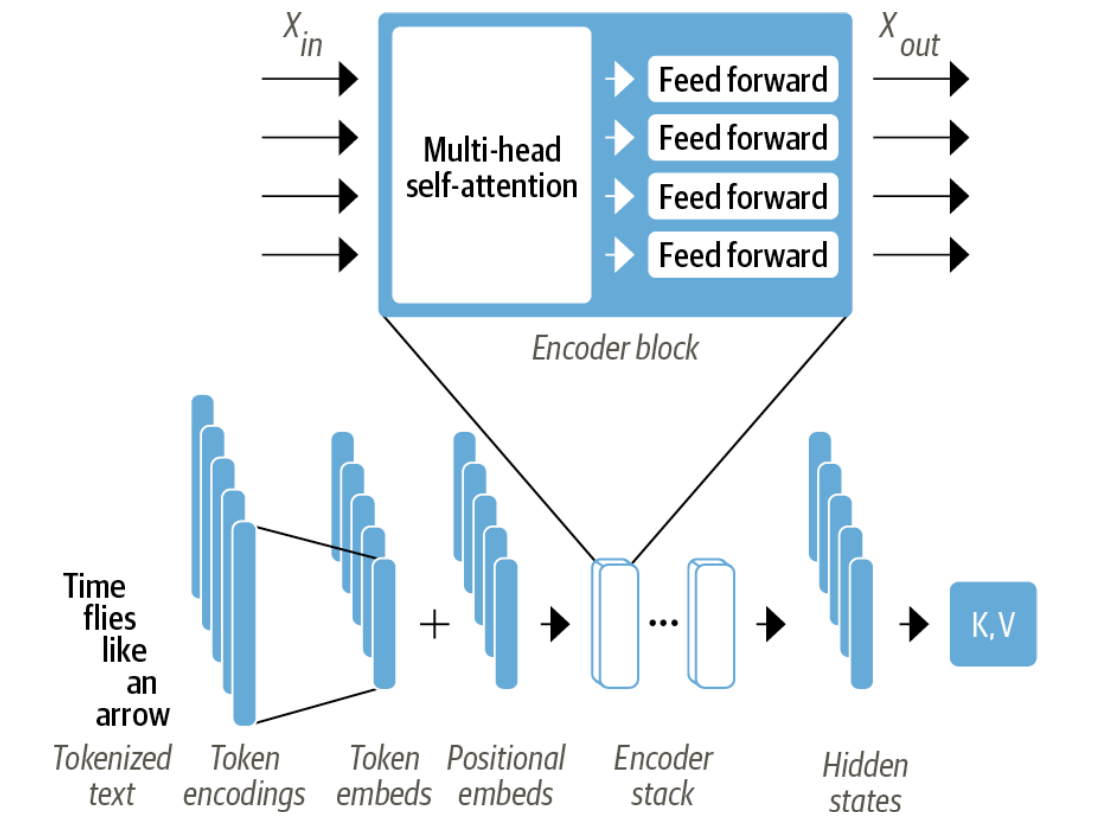
\includegraphics[height=80mm]{graphics/encoder-block.png}
    \caption[Aufbau eines Encoder-Blocks]{Aufbau eines Encoder-Blocks \footnotemark}
    \label{fig:encoder-block}
\end{figure}
\footnotetext{Entnommen aus: \cite{tunstall_natural_2022}, S.60}
%TODO: Complete Chapter: Decoder, Zusammenspiel, Bottleneck -> Relevanz Attention



%%% Ende des eigentlichen Inhalts %%%

% chapter  (end)

%%% Quellenverzeichnisse (keine Anpassung nötig) %%%
\clearpage
\literaturverzeichnis
%%% Ende Quellenverzeichnisse %%%

\clearpage
\clearpage

\thispagestyle{empty}

{\LARGE\textsf{\textbf{Erklärung zur Verwendung generativer KI-Systeme}}\bigskip}

Bei der Erstellung der eingereichten Arbeit habe ich die nachfolgend aufgeführten auf künstlicher Intelligenz (KI) basierten Systeme benutzt:
% HIER EDITIEREN: (Immer mit \item einen neuen Antrag anführen
\begin{enumerate}
  \item
\end{enumerate}

Ich erkläre, dass ich
\begin{itemize}
  \item mich aktiv über die Leistungsfähigkeit und Beschränkungen der oben genannten KI-Systeme informiert habe, \footnote{U. a. gilt es hierbei zu beachten, dass an KI weitergegebene Inhalte ggf. als Trainingsdaten genutzt und wiederverwendet werden. Dies ist insb. für betriebliche Aspekte als kritisch einzustufen.}
  \item die aus den oben angegebenen KI-Systemen direkt oder sinngemäß übernommenen Passagen gekennzeichnet habe, \footnote{In der Fußnote Ihrer Arbeit geben Sie die KI als Quelle an, z.B.: Erzeugt durch Microsoft Copilot am dd.mm.yyyy. Oder: Entnommen aus einem Dialog mit Perplexity vom dd.mm.yyyy. Oder Absatz 2.3 wurde durch ChatGPT sprachlich geglättet.}
  \item überprüft habe, dass die mithilfe der oben genannten KI-Systeme generierten und von mir übernommenen Inhalte faktisch richtig sind, \footnote{Beispiele hierfür sind u.a. die folgenden Arbeitsschritte: Generierung von Ideen, Konzeption der Arbeit, Literatursuche, Literaturanalyse, Literaturverwaltung, Auswahl von Methoden, Datensammlung, Datenanalyse, Generierung von Programmcodes.}
  \item mir bewusst bin, dass ich als Autorin bzw. Autor dieser Arbeit die Verantwortung für die in ihr gemachten Angaben und Aussagen trage.
\end{itemize}

\vspace{1cm}

Die oben genannten KI-Systeme habe ich wie im Folgenden dargestellt eingesetzt:
\begin{center}
  \begin{tabular}{| p{0.25\linewidth} | p{0.2\linewidth} | p{0.5\linewidth} |}
    \hline
    \textbf{Arbeitsschritt in der wissenschaftlichen Arbeit} & \textbf{Eingesetzte(s) KI-System(e)} & \textbf{Beschreibung der Verwendungsweise} \\
    \hline
    % HIER EDITIEREN: (Nächste Zeile beliebig oft kopieren)
                                                             &                                      &                                            \\
    \hline
  \end{tabular}
\end{center}



%%% Erklärung (keine Anpassungen nötig) %%%
% steht ganz am Ende des Dokuments
\cleardoublepage
\clearpage

\thispagestyle{empty}

{\LARGE\textsf{\textbf{Erklärung}}\bigskip}

% \typMeinerArbeit und \themaMeinerArbeit werden in deckblatt.tex definiert
Ich versichere hiermit, dass ich die vorliegende Arbeit mit dem Thema: \emph{\themaMeinerArbeit} selbstständig verfasst und keine anderen als die angegebenen Quellen und Hilfsmittel benutzt habe.
Ich versichere zudem, dass die eingereichte elektronische Fassung mit der gedruckten Fassung übereinstimmt.

\vspace{3cm}

\begin{center}
  \begin{tabular}{ccc}
    (Ort, Datum) & \hspace{0.3\linewidth} & (Unterschrift)
  \end{tabular}
\end{center}
\end{document}
